\chapter{Theoretical Background}\label{chapter:theoreticalBackground}
To critically assess the impact of globalization on economic inequality, it is essential to first establish a clear understanding of the key concepts and theoretical frameworks that underpin this analysis. This section will define and explore the concepts of globalization and economic inequality, as well as review relevant economic theories that explain the interaction between these two phenomena.

\section{Globalization}\label{globalization}

The term “globalization” became more widely used in the 1980s, driven by technological advancements that facilitated faster and more efficient international trade and financial transactions. Globalization, which is commonly defined as the movement of goods, services, capital, people, information, and ideas across borders, has significantly progressed in recent decades. A book by \citep{held2003globalizationDebate} interestingly defines globalization as " the expanding scale, growing magnitude, speeding up and deepening impact of interregional flows and patterns of social interaction" and "a shift or transformation in the scale of human social organization that links distant communities and expands the reach of power relations across the world's major regions and continents." This process has led to increased integration of economies and societies, making it a prominent and seemingly unavoidable aspect of the modern world \citep{agenor2002globalizationPoor}.

Globalization refers to the process by which national economies, societies, and cultures have become increasingly integrated and interdependent due to the rapid exchange of goods, services, information, and capital across borders. This phenomenon has been driven by advancements in transportation, communication technologies, and trade liberalization policies, which have facilitated the movement of resources and knowledge on a global scale \citep{Held1999globalTransformations}. Economically, globalization is often associated with the rise of multinational corporations, global supply chains, and increased international trade and investment. These elements have led to greater economic integration, enabling countries to specialize in the production of goods and services that align with their comparative advantages \citep{krugman2010internationalEconomics}. However, this integration has also created vulnerabilities, as economies have become more susceptible to global market fluctuations and external shocks. Figure \ref{fig:globalizationOver5Centuries} shows the globalization over the last 5 centuries through the "trade openness index" expressed by the sum of world exports and imports, divided by world GDP.
\begin{figure}[H]
    \centering
    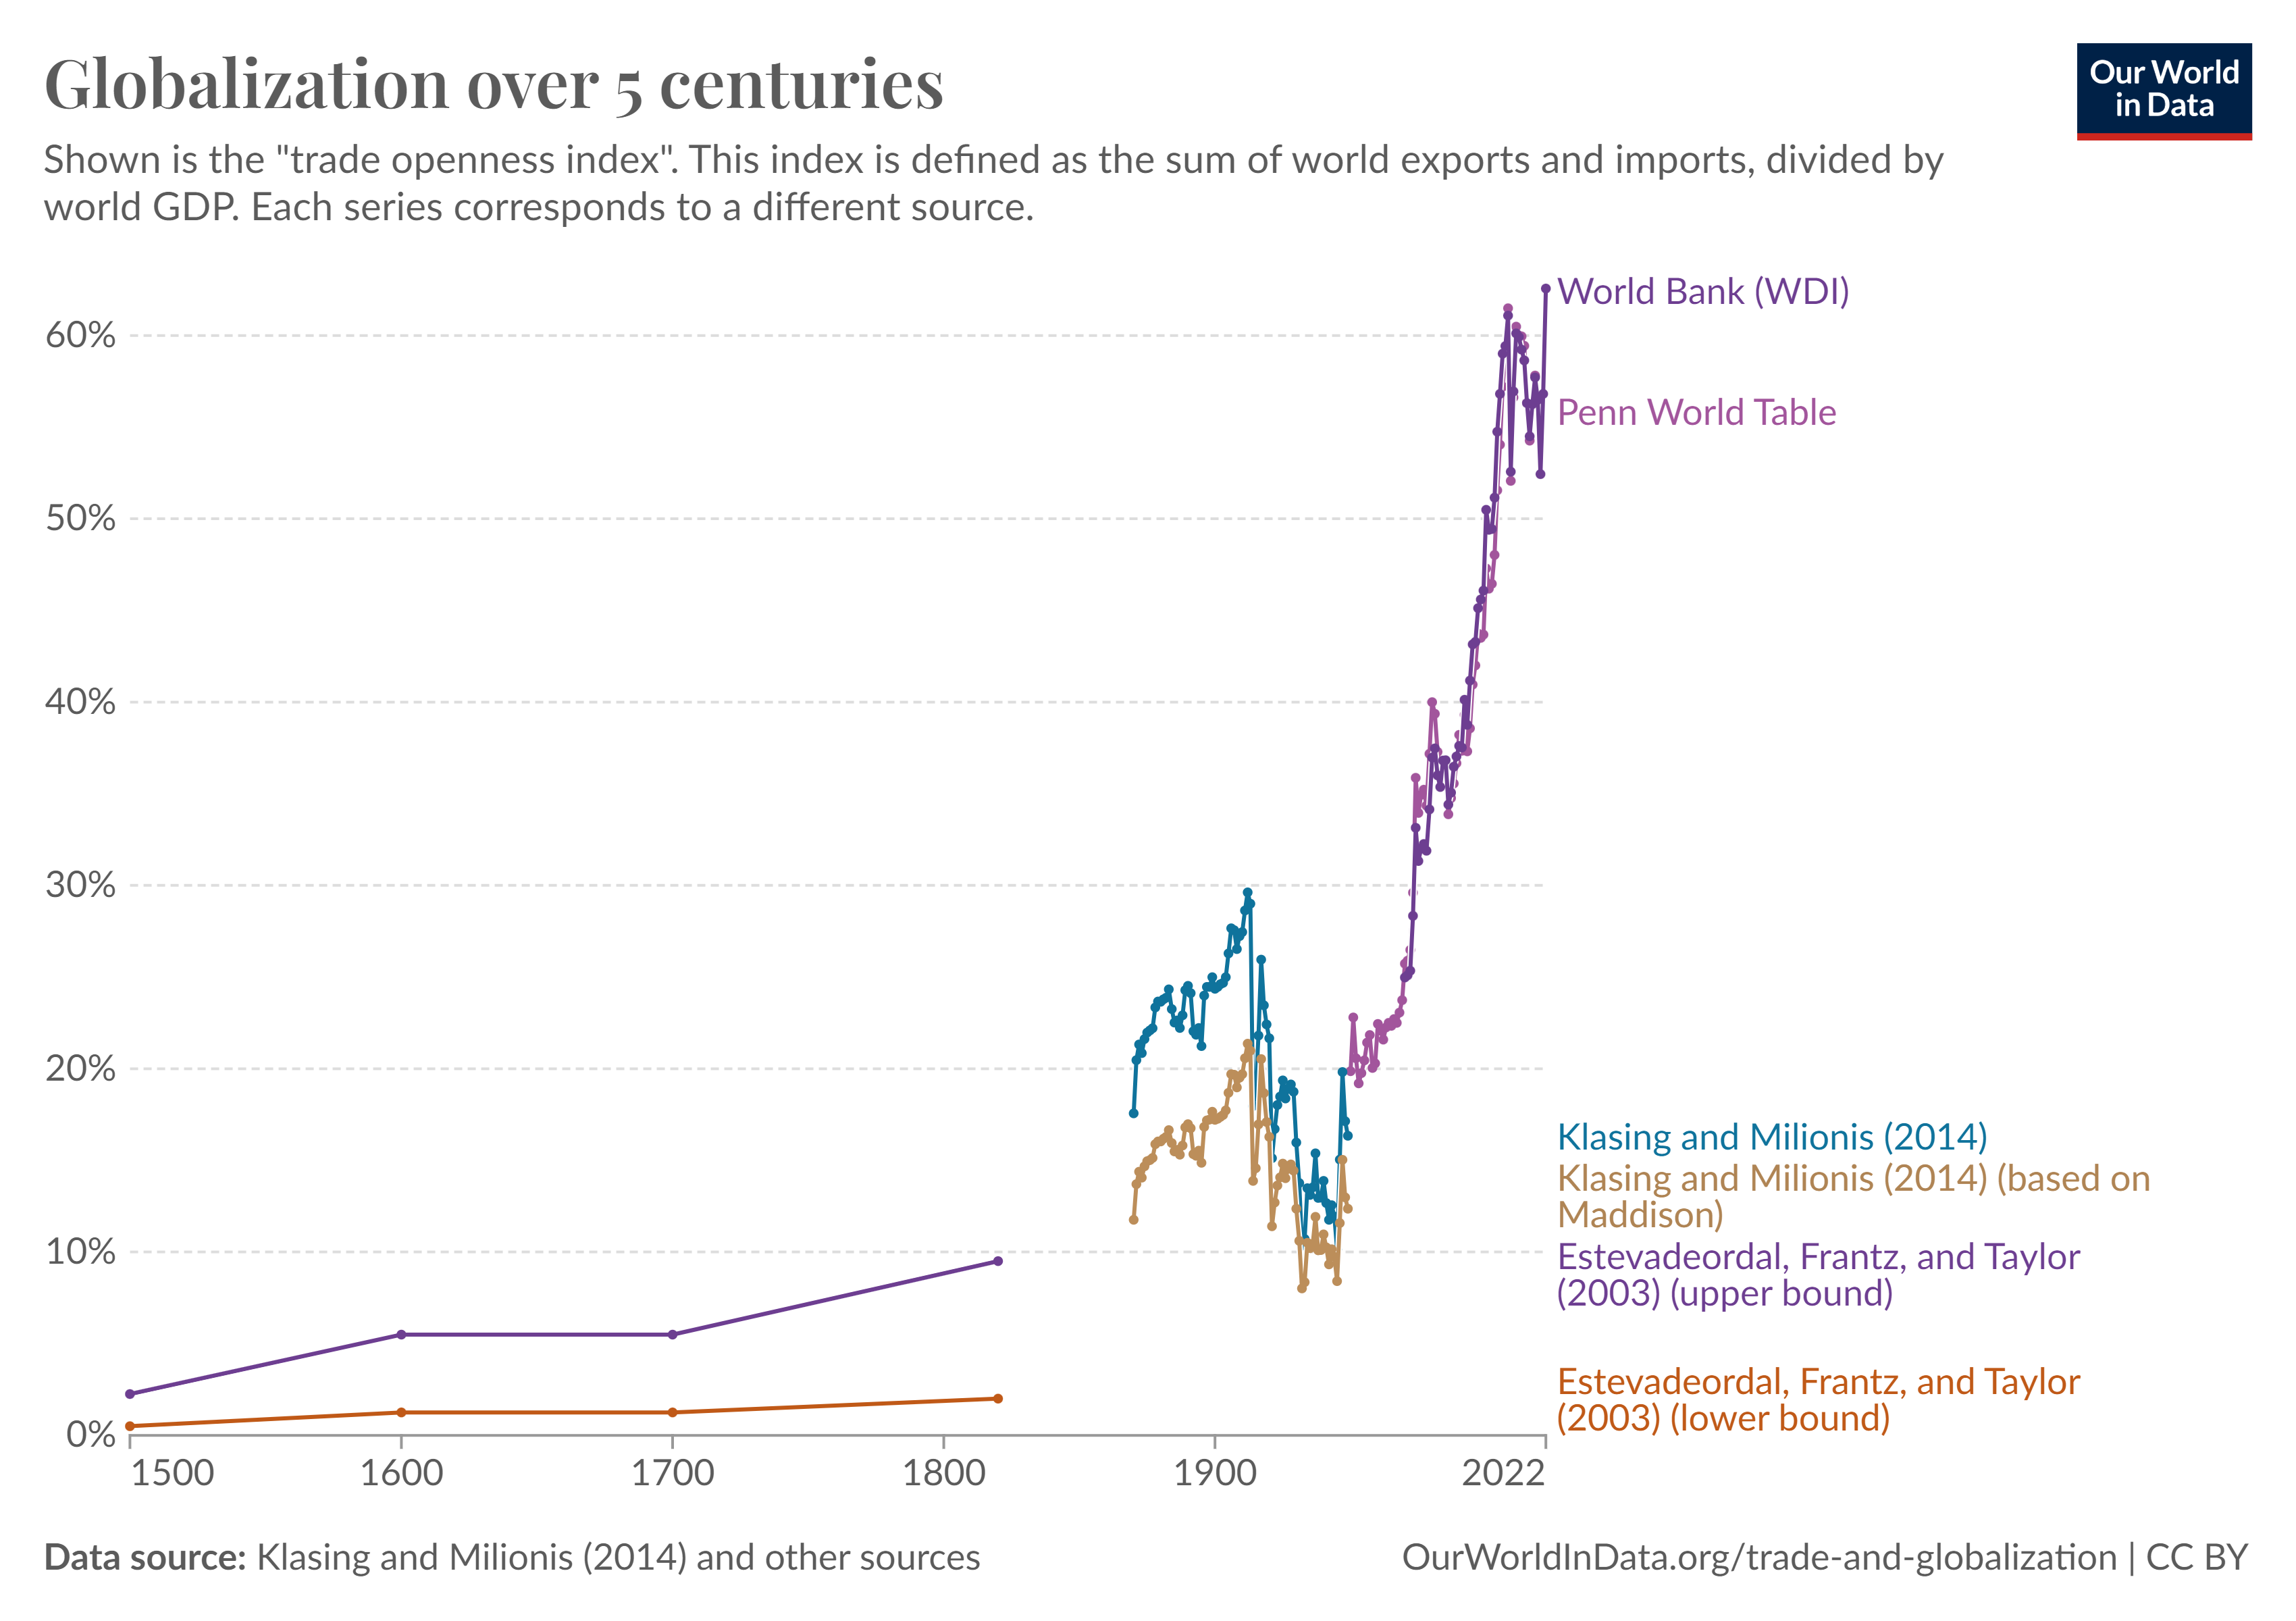
\includegraphics[scale=0.1]{globalization-over-5-centuries.png}
    \caption{Globalization over 5 centuries}
    \label{fig:globalizationOver5Centuries}
    \citep{ourWorldInData2023globalization5centuries}
\end{figure}

The concept of globalization encompasses various dimensions, including economic, political, cultural, and technological, each of which contributes to the deepening of global connections. Theoretically, globalization is driven by several factors \citep{thompson2023factors}, including:
\begin{itemize}
    \item \textbf{Technological advancements:} Innovations in transportation and communication technologies have significantly reduced the costs of doing business across borders. The transport sector’s efficiency saw significant improvements with the advent of multimodal transport, which integrates maritime and surface transportation. This development enhanced connectivity within countries and with neighboring nations, facilitated by highways and roads. The rise of digital platforms and e-commerce has transformed how businesses operate and reach global markets. Instant communication and online transactions have made cross-border trade more accessible.
    \item \textbf{Reduced trade barriers:} Governments have lowered tariffs, quotas, and other trade restrictions, facilitating the flow of goods and services between countries. The reduction of trade barriers, such as tariffs and quotas, has facilitated the free flow of goods and services across borders. This has been supported by international trade agreements and organizations.
    \item \textbf{The rise of multinational corporations:} Businesses with operations in multiple countries have played a crucial role in driving globalization by investing in foreign markets and economies of scale.
    \item \textbf{Financial liberalization:} Deregulation of financial markets has allowed for the free movement of capital across borders, promoting cross-border investments and trade.
\end{itemize}

\section{Economic Inequality}\label{economicInequality}

Economic inequality refers to the unequal distribution of income and wealth within and between populations. It can manifest in various forms, including income inequality, wealth inequality, and disparities in access to education, healthcare, and opportunities. Economic inequality is typically measured using indices such as the Gini coefficient, which quantifies the degree of inequality on a scale from 0 (perfect equality) to 1 (maximum inequality) (Deininger \& Squire, 1996).

Theoretical perspectives on economic inequality have evolved over time. Classical economists like Adam Smith and David Ricardo acknowledged the existence of inequality but emphasized the role of free markets in promoting efficiency and growth. In contrast, Marxist theories highlighted the exploitative nature of capitalism, where wealth accumulates in the hands of a few, leading to systemic inequality (Marx, 1867). More recent theories, such as those proposed by Piketty (2014), suggest that the dynamics of capital accumulation in a globalized economy tend to exacerbate inequality, as returns on capital often outpace economic growth.


\section{Globalization and Economic Inequality}\label{globalizationEconomicInequality}

Economic development has benefited from increased globalization, but this has also come at the cost of greater income inequality between countries.
The relationship between globalization and income inequality is a complex and 
multifaceted issue that has attracted considerable attention from scholars, policymakers, and the general public. As economies become more integrated into the global system, questions arise about the distributional consequences of this process. The overarching aim of this research paper is to conduct a comprehensive analysis of the impact of globalization on income inequality, delving into the nuanced dynamics that underlie this relationship.
Historically, the discourse surrounding globalization and income inequality has been polarized, with divergent views on the extent and nature of their correlation. Some argue that globalization fosters economic growth, leading to a rise in overall income levels and, consequently, a reduction in poverty. Conversely, critics contend that globalization exacerbates income inequality by favoring certain segments of the population, often those with access to capital and skills, while leaving others behind.

